\documentclass{standalone}
\usepackage{ tikz }
\usetikzlibrary{shapes}
\usetikzlibrary{plotmarks}
\usepackage{amsmath}
\usepackage{ xparse }
\usepackage{../../../macros}

\begin{document}
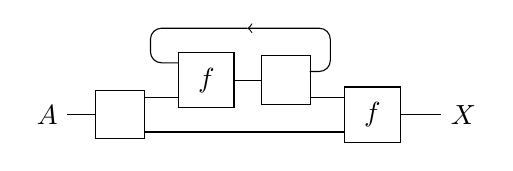
\begin{tikzpicture}[yscale=-1,x=1em,y=1.25em]
        
    \node [anchor=east] at (10.5,0) {$A$};
    \draw (10.5, 0) -- (11.5,0);
    \node[draw, minimum height = 1.75em, minimum width = 1.75em, anchor = west] at (11.5,0){$\ccopy{}$};
    \draw [rounded corners] (13.25,-0.5) -- (14.5, -0.5);
    \draw [rounded corners] (13.25,0.5) -- (20.5,0.5);
    \node[draw, minimum height = 2em, minimum width = 2em, anchor = west] at (14.5,-1){$f$};
    \draw (16.5,-1) -- (17.5,-1);
    \node[draw, minimum height = 1.75em, minimum width = 1.75em, anchor = west] at (17.5,-1){$\ccopy{}$};
    \draw [->, rounded corners] (19.25,-1.25) -- (20,-1.25) -- (20, -2.5) -- (17, -2.5);
    \draw [rounded corners] (17, -2.5) -- (13.5,-2.5) -- (13.5, -1.5) -- (14.5,-1.5);
    \draw [rounded corners] (19.25,-0.5) -- (20.5,-0.5);
    \node[draw, minimum height = 2em, minimum width = 2em, anchor = west] at (20.5,0){$f$};
    \draw (22.5,0) -- (24,0);
    \node [anchor=west] at (24,0) {$X$};

\end{tikzpicture}
\end{document}